\subsection{Prerequisites Installation}
The ITD provided by the group under analysis properly covers the installation guide for the software prerequisites.
The software in question is:
\begin{itemize}
    \item Windows Subsystem for Linux 2 (WSL2):\\
         a compatibility layer that enables running a full Linux kernel on Windows. It is needed to be able to install and use the next prerequisite;
    \item Docker Desktop:\\
    an application that enables running and managing Docker containers on Windows, integrating WSL 2 for improved performance and native Linux compatibility.
    \item Node.js:\\
    a JavaScript runtime built on Chrome's V8 engine that allows executing JavaScript code outside the browser, enabling backend development and server-side applications.
\end{itemize}
Since these are very common tools and pieces of software, widely used by developers, their installation was not necessary, as our systems already had them installed and set up.

\subsection{Backend Environment Set Up}

In the \verb|backend| directory, there are all the needed files to properly configure the backend services. The "\verb|docker-compose.yaml|" file defines four services:
\begin{itemize}
    \item Postgres service:\\
        Database;
    \item Adminer service: \\
        Database Manager with UI;
    \item Mail service:\\
        SMTP server for sending email in a dev environment;
    \item API service:\\
        the service responsible to run the node server derving the business logic api.
\end{itemize}

As specified by the ITD, the only services that shall run in separated containers are the first three as the api one shall be run locally, ignoring the docker compose setup defined for it. 



\subsubsection*{Installation Steps}

The steps we executed once in the main project directory are:
\begin{enumerate}
    \item Navigate to the \verb|backend| directory:
        \begin{verbatim}
            cd backend
        \end{verbatim}
\item Install the Node.js project dependencies:
        \begin{verbatim}
            npm install
        \end{verbatim}
\item Run the three docker containers:
        \begin{verbatim}
            docker compose up -d postgres adminer maildev
        \end{verbatim}
The \verb|-d| argument lauch the containers in detached mode meaning the terminal will still be available to run other commands (while by default it keeps showing the docker logs)
\item Install api server dependencies:
        \begin{verbatim}
            npm install
        \end{verbatim}
\item Execute the npm script to construct the database:
        \begin{verbatim}
            npm run migration:run
        \end{verbatim}
\item Seed the database:
        \begin{verbatim}
            npm run seed:run:relational
        \end{verbatim}
\item Start the server locally on our device:
        \begin{verbatim}
            npm run start:dev
        \end{verbatim}
\end{enumerate}

\subsubsection*{Result}
After executing all the previous commands, we have three containers running the following services:
\begin{itemize}
    \item Postgres service:\\
        Database;
    \item Adminer service: \\
        Database Manager with UI;
    \item Mail service:\\
        SMTP server for sending email in a dev environment;
\end{itemize}

\begin{figure}[H]
    \centering
    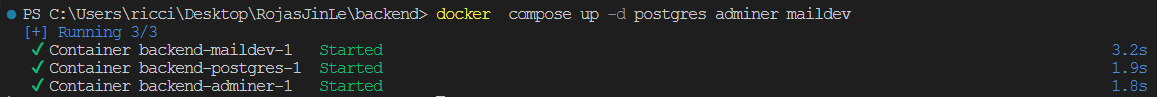
\includegraphics[width=1\linewidth]{Latex/Images/ATD/containers.png}
    \caption{Running Containers}
    \label{fig:containers}
\end{figure}

And the api server running on directly on our device OS ready to serve on \verb|localhost:3000|:

\begin{figure}[H]
    \centering
    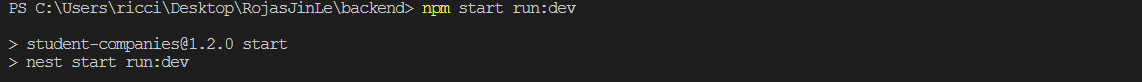
\includegraphics[width=1\linewidth]{Latex/Images/ATD/npmrun.png}
    \caption{Running API server}
    \label{fig:containers}
\end{figure}



\subsection{Frontend Environment Set Up}
As the prototype client is an Android application we need an emulator to be able to test it. The ITD specify to use the Android Studio IDE emulator to run the application; so we installed it on our devices.
The ITD also provided us with a link to a cloud storage containing the build of the client app that we downloaded and copied into the emulator.

\subsubsection*{Installation Steps}
\begin{enumerate}
    \item Install Android Studio IDE from its website;
    \item Create a new android device emulator and start it;
    \item Download the client build file from the cloud storage link;
    \item Copy the build file into the running emulator
    \item Open the client application;
\end{enumerate}

\subsubsection*{Result}
The result is a running portable android device emulator containing the client application ready for testing.


\begin{figure}[H]
    \centering
    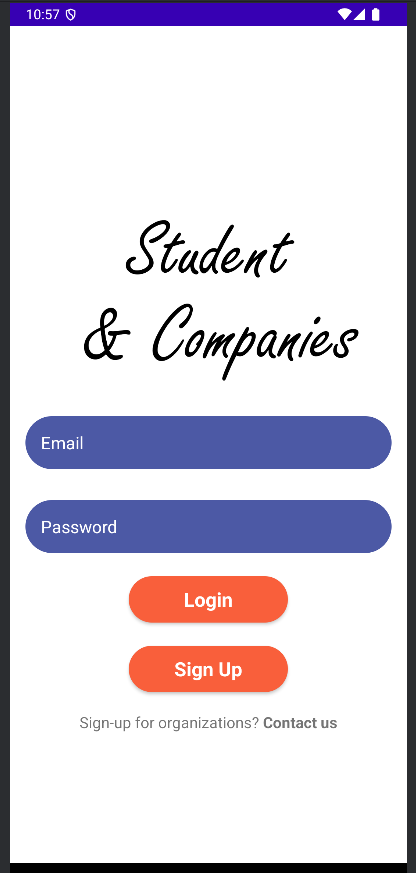
\includegraphics[width=0.3\linewidth]{Latex/Images/ATD/AndroidApp.png}
    \caption{Android Emulator running the client App}
    \label{fig:androidapp}
\end{figure}




